\documentclass{report}

\usepackage{graphicx}
\usepackage{float}
\usepackage{wrapfig}
\usepackage{color}
\usepackage{siunitx}
\usepackage[usenames,dvipsnames]{xcolor}
\usepackage[english]{babel}
\usepackage{amssymb}
\usepackage{geometry}

\begin{document}

\title{\textbf{Homework 2:} Random Numbers and Multidimensional Monte-Carlo Integration}
\author{A.L. Phillips II\\
  Department of Physics, Astronomy, and Applied Physics,\\
  Rensselaer Polytechnic Institute\\
  \texttt{philla3@rpi.edu}}
 \date{27 February 2013}
 \renewcommand{\chaptername}{Assignment}
 \setcounter {chapter}{1}
\maketitle

\chapter{Random Numbers and Multidimensional Monte-Carlo Integration}

\section{Pseudo Random}
\begin{enumerate}
\item The term "random number" is largely a misnomer when referring to numbers generated by machines.  Machine algorithm is intrinsically deterministic and it is for this reason that numbers generated in such a manner are termed pseudo random numbers. Pseudo random number generators (PRNG) cannot be "truly" random, however, they may have the appearance of being so over a specific period. PRNG's can be assessed by their ability to mask their period of repetition when producing quantities of PRN's that are comparable to the generators period. In this section, the discussion of PRNG's will includes examples from the Power-Residue method, rand48() and random.org distributions. Below, Figures~\ref{rand48} and~\ref{randOrg} each provide "$PRN vs i$" plots respectively.
\\
\begin{figure}[H]
\centering \caption{15,000 Pseudo Random Numbers using rand48()}
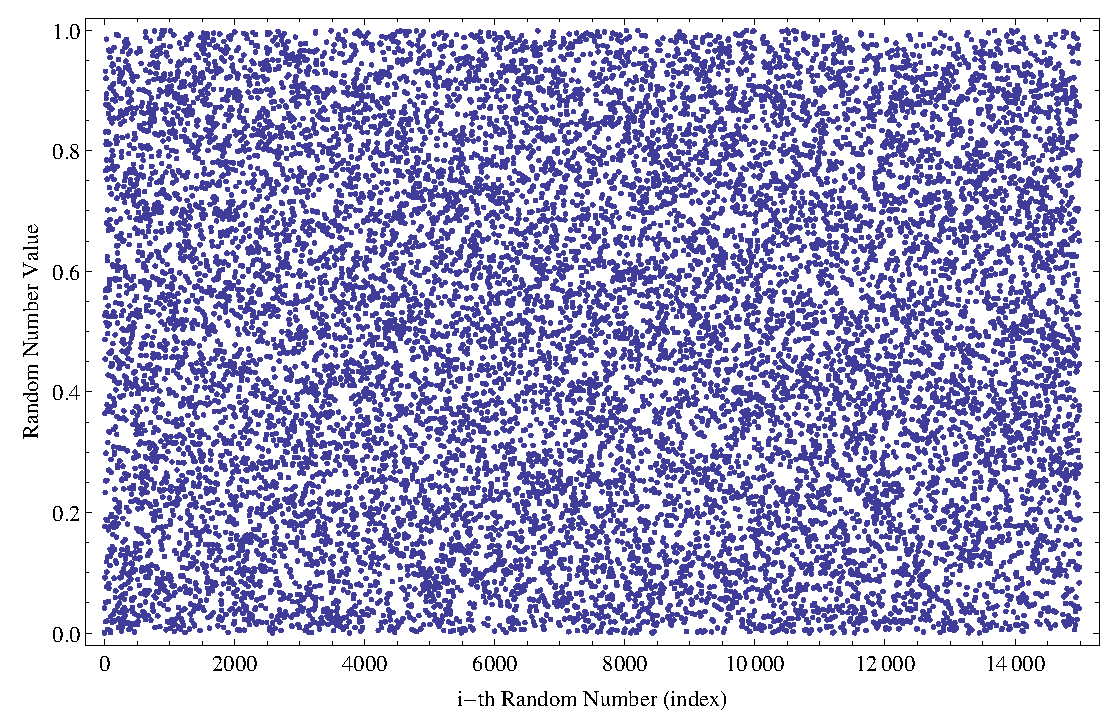
\includegraphics[scale=.42]{drand48.eps}
\label{rand48}
\end{figure}

\begin{figure}[H]
\centering \caption{10,000 Random Numbers from http://random.org}
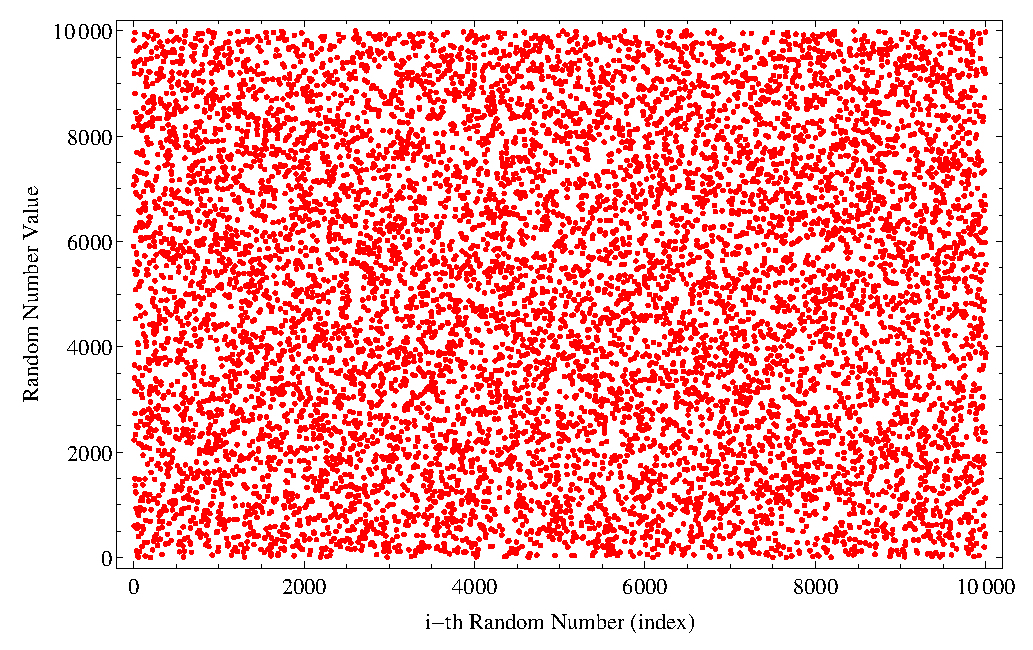
\includegraphics[scale=.7]{randomOrg.eps}
\label{randOrg}
\end{figure}

Qualitative Analysis:
\\
\\The usefulness of a PRNG may be determined by assessing the uniformity and non-correlation of its plot(s). By "uniformity", it is meant that the plot of PRN's is uniformly distributed throughout it's plot. By "non-correlation", it is meant that there appears no pattern or correlation between the PRN's. These criteria may be assessed qualitatively by the user visually inspecting the PRNG's plots for uniformity and non-correlation. Notice then that the drand48() and random.org plots in Figures~\ref{rand48} and ~\ref{randOrg} both pass the visual uniformity and non-correlation tests.
\\
\\ To contrast the successful tests above, Figure~\ref{powerResidue} depicts the Power-Residue PRNG failing the visual inspection. Notice that while the Power-Residue method appears well distributed, the correlation between it's PRN's are visually simple to identify. 
\\
\begin{figure}[H]
\centering \caption{15,000 Shameful Pseudo Random Numbers using Power-Residue method}
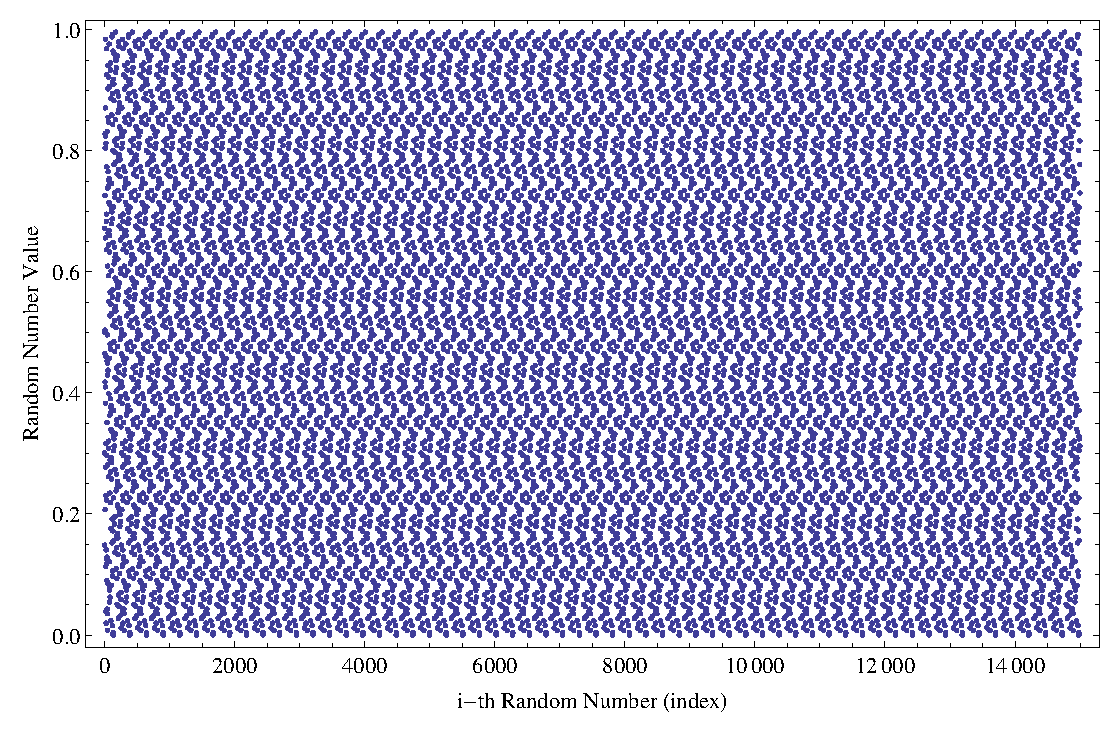
\includegraphics[scale=.6]{powerResidue.eps}
\label{powerResidue}
\end{figure} 
Another method of qualitatively assessing non-correlation is to plot " $\displaystyle x_i$ vs $\displaystyle x_{i+k}$ " where $x_i$ is the $i^{th}$ random number and $k$ is a "small" value which shifts the index. This plot may allow us to visually detect correlation that was not previously evident in the  plot of " $\displaystyle i$ vs $\displaystyle x_{i}$ ". Figure ~\ref{xixik} represents what the " $\displaystyle x_i$ vs $\displaystyle x_{i+k}$ " plots look like for both the drand48() and random.org distributions.
\\
\\\begin{figure}[H]
\centering \caption{Depiction of "$\displaystyle x_i$ vs $\displaystyle x_{i+k}$" plots for both drand48() and random.org}
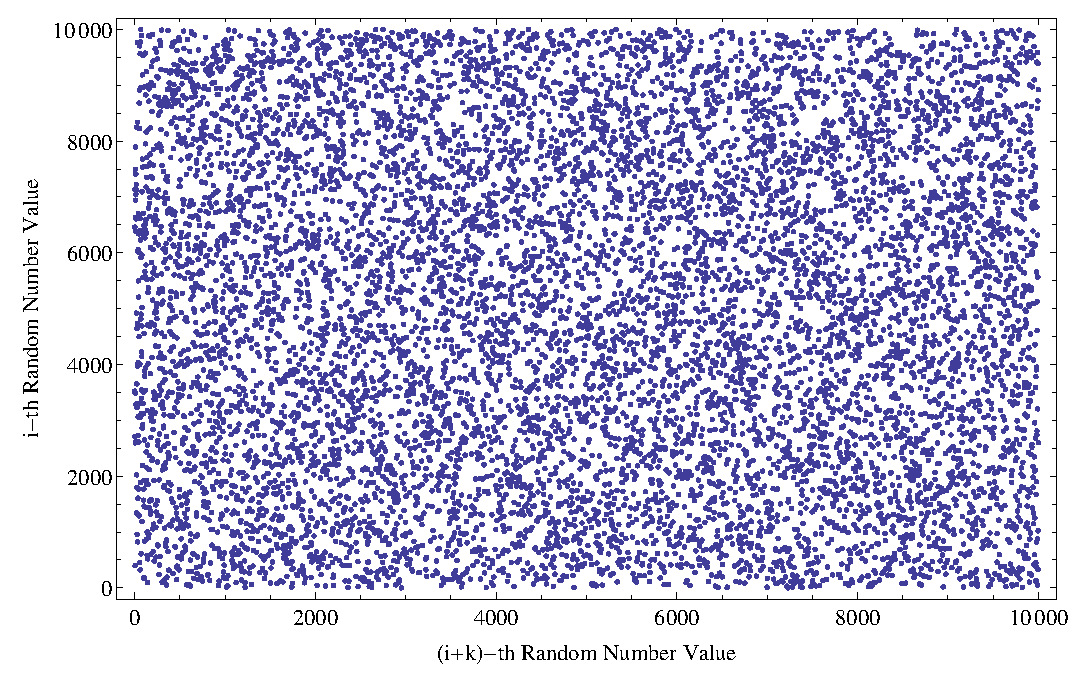
\includegraphics[scale=.7]{drand48()XIXIK.eps}
\label{xixik}
\end{figure}
Notice that the "$\displaystyle x_i$ vs $\displaystyle x_{i+k}$" plot appears identical to the original "$\displaystyle i$ vs $\displaystyle x_{i}$" plots. Because of this, we gain confidence in each PRNG's ability to produce, "random", uniform distributions. 
\\
\\To contrast this this result, Figure~\ref{powerResK} shows the Power-Residue PRNG's "$\displaystyle x_i$ vs $\displaystyle x_{i+k}$" plot. We've already determined that the Power-Residue method fails the visual correlation criterion in Figure~\ref{powerResidue}" and so the pattern evident in Figure~\ref{powerResK} is expected.
\begin{figure}[H]
\centering \caption{Shameful "$\displaystyle x_i$ vs $\displaystyle x_{i+k}$" plot for Power Residue Method}
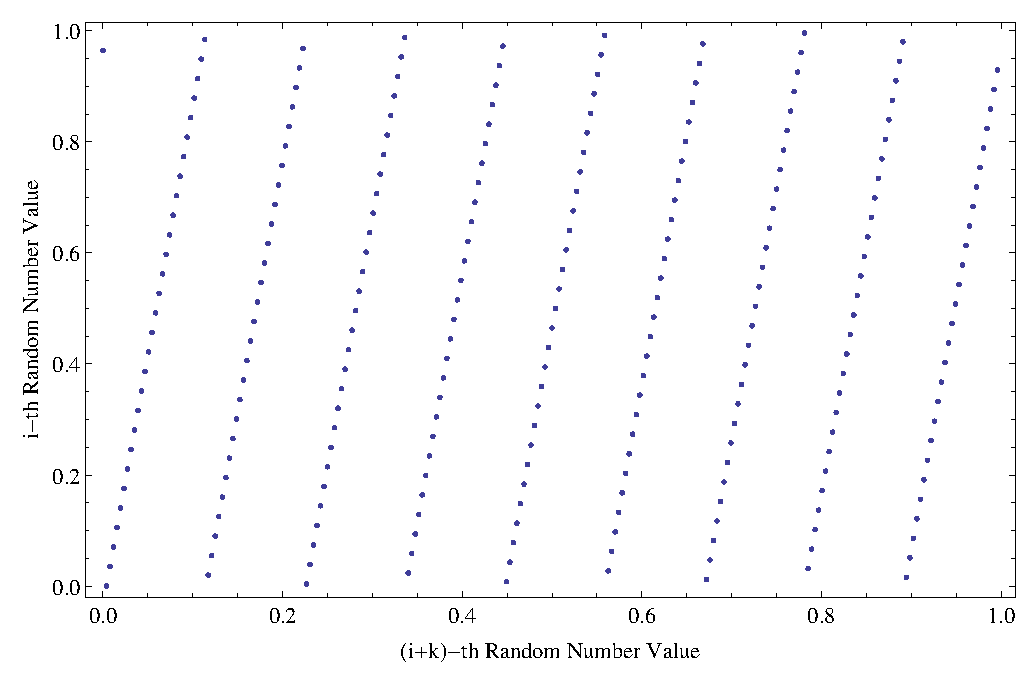
\includegraphics[scale=.63]{powerResidueXIXIK.eps}
\label{powerResK}
\end{figure}
Histograms are another method by which the uniformity of a distribution may be visualized. This is done by dividing the sample range into intervals known as bins. For example, we used drand48() to calculate 15,000 PRN's in the range of $[0,1]$. If we divide this range into 10 intervals, each bin in the x-axis of the histogram would be equal to $0.1$. The distributions PRN's are each placed into their respective bin, whereby a histogram displaying the distributions uniformity is produced. If each bin has an equal number of PRN's, the top of the bins will all align and the distribution is considered uniform. The more offset between bins, the less uniform the distribution.
\\
\\Figures~\ref{randHistogram} and~\ref{randOrgHistogram} provide histograms of drand48()'s and random.org's distributions. Notice the unevenness in drand48()'s histogram as opposed to random.org's. These histograms suggest that random.org's distribution is absolutely uniform whereas drand48()'s is close, but not perfect.
\begin{figure}[H]
\centering \caption{drand48() 10-Bin Histogram}
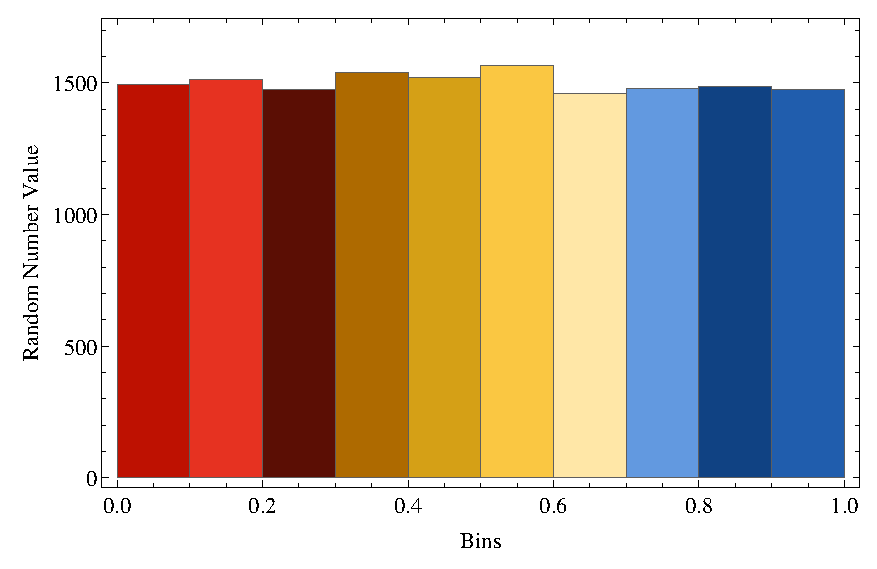
\includegraphics[scale=.6]{randHistorgram.eps}
\label{randHistogram}
\end{figure} 

\begin{figure}[H]
\centering \caption{random.org 10-Bin Histogram}
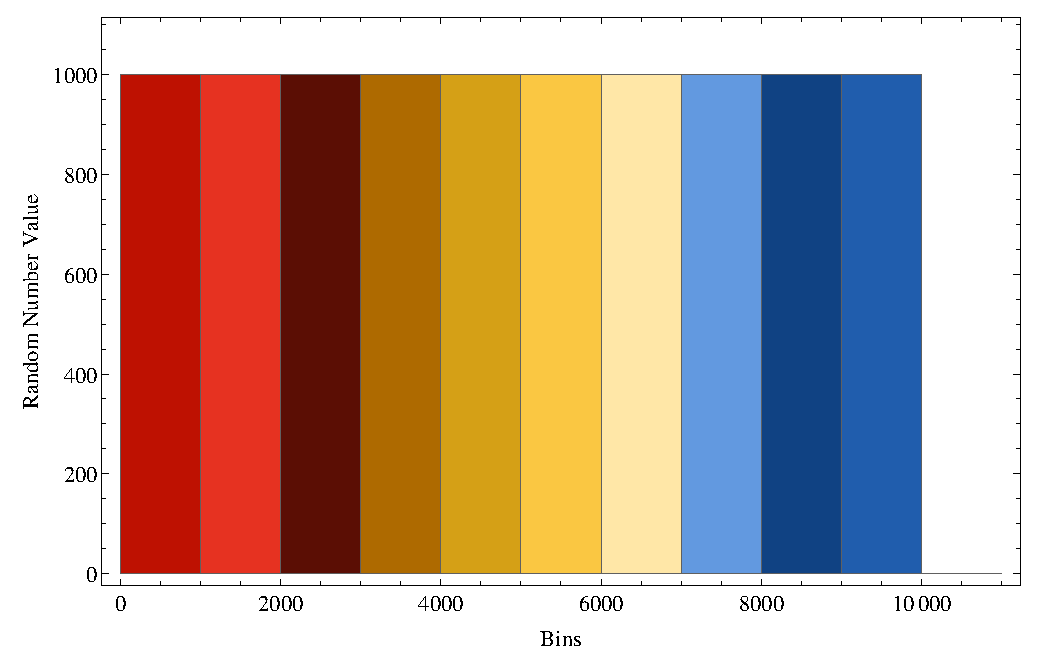
\includegraphics[scale=.5]{randOrgHist.eps}
\label{randOrgHistogram}
\end{figure} 
Quantitative Analysis:
\\
\\
\\The above methodologies take advantage of our ability to qualitatively assess uniformity and non-correlation. While these tests are effective and an ease to implement, there exist numerous quantitative measures as discussed below:
\\
\\
\\The $k^{th}$-moment:
\\
\\
\\The $k^{th}$ moment test of a PRN distribution addressees uniformity. If a PRNG produces uniformly distributed PRN's, then the average of all of the PRN's raised to a sufficiently small $k$ should approximate $\frac{1}{k+1}$. That is:
\\
\begin{equation}
\frac{1}{N} \sum\limits_{i=1}^n x_i^k \approx \frac{1}{k+1}
\end{equation}
Note: If the standard deviation (average distance from the average point) varies as $\displaystyle \frac{1}{N}$, then the distribution may be considered "random".
\\
\\
\\
\\Below are the $k^{th}$ moment calculations for the rand48() and random.org distributions:
\\
.\hspace{30 mm}
$\displaystyle rand48(): \hspace{5 mm}
\frac{1}{\SI{1.5e4}{}} \sum\limits_{i=1}^{\SI{1.5e4}{}} x_i^{4} \approx \frac{1}{4+1}$
\\
\\
.\hspace{35 mm}
$\displaystyle \hspace{18 mm}
0.198068074284546 \approx 0.2$
\\
\\
.\hspace{5 mm} Relative Error between Calculated and Theoretical $k^{th}$ moments = 0.0097538471
\\
\\
\\
\\.\hspace{20 mm}
$\displaystyle random.org \hspace{5 mm}
\frac{1}{\SI{1e4}{}} \sum\limits_{i=1}^{\SI{1e4}{}} x_i^{\SI{4e-5}{}} \approx \frac{1}{\SI{4e-5}{}+1}$
\\
\\
.\hspace{43 mm}
$\displaystyle \hspace{18 mm}
1.0003284904 \approx 0.9999600016$
\\
\\
.\hspace{5 mm} Relative Error between Calculated and Theoretical $k^{th}$ moments = 0.0003685036
\\
\\
\\
\\Notice here the significant decrease in error that random.org's distribution displays over drand48() --Nearly $2$ orders of magnitude less error! These results depict the strong non-correlation advantage of the random.org distribution.
\\
\\Auto Correlation (Near-neighbor Correlation):
\\
\\
\\Auto correlation tests non-correlation between PRN's within a distribution. If a PRNG produces uniformly distributed PRN's, then the average of all $x_i x_{i+k}$ PRN's should approximate $\frac{1}{4}$. More specifically, the formula for Auto Correlation is as follows:
\\
\begin{equation}
\frac{1}{N} \sum\limits_{i=1}^n x_i x_{i+k} \approx \frac{1}{4}
\end{equation}
Note: The standard deviation (average distance from the average point) varying as $\displaystyle \frac{1}{N}$ ensures that the distribution is "random".
\\
\\
\\
\\Below are Auto Correlation calculations for the rand48() and random.org distributions:
\\
\\
.\hspace{30 mm}
$\displaystyle rand48(): \hspace{5 mm}
\frac{1}{\SI{1.5e4}{}} \sum\limits_{i=1}^{\SI{1.5e4}{}} x_i x_{i+1} \approx \frac{1}{4}$
\\
\\
.\hspace{35 mm}
$\displaystyle \hspace{22 mm}
0.248318844894805 \approx 0.25$
\\
\\
.\hspace{5 mm} Relative Error between Calculated and Theoretical Auto Correlations = 0.006724620420
\\
\\
\\.\hspace{20 mm}
$\displaystyle random.org: \hspace{5 mm}
\frac{1}{\SI{1e4}{}} \sum\limits_{i=1}^{\SI{1e4}{}} x_i x_{i+0.00004} \approx \frac{1}{4}$
\\
\\
.\hspace{43 mm}
$\displaystyle \hspace{16 mm}
0.248989071076 \approx 0.25$
\\
\\
.\hspace{5 mm} Relative Error between Calculated and Theoretical Auto Correlations = 0.004043715696
\\
\\
\\Notice here the decrease in error that random.org's distribution displays over drand48() --While the difference in error is not as significant as in the $k^{th}$ moment calculations, the results still display a non-correlation advantage in random.org's distribution.
\\
\\
\\
\\
\\
\\
\end{enumerate}



\section{Multidimensional Monte-Carlo Integration}


\begin{enumerate}
\item The Monte-Carlo integration method is a technique used for numerically approximating the area under an n-dimensional function. The method is implemented much alike the mean value theorem. The two methods are similar in that they both use the limits of integration ($b-a$) as the width in the area calculation. Where the methods differ is in Monte-Carlo's application of random numbers to determine the height in the area calculation. The height is determined by taking $N$ evenly distributed random numbers, inputting them into the given function, and averaging their resulting values.
\\
\\The formula for a multidimensional Monte Carlo integral is as follows: 
\begin{equation}
\int_a^b \int_c^d \int_e^f f(x_1,x_2,x_3) dx_1 dx_2 dx_3 \approx (b-a)(d-c)(f-e)\frac{1}{N} \displaystyle\sum\limits_{i=0}^N f(x_i)
\end{equation}

Here, "$f(x_1,x_2,x_3)$" is a surface in $\mathbb{R}^3$ , the variables in "$(b-a)(d-c)(f-e)$" correlate directly to the limits of integration and "$N$" represents the number of iterations/random numbers used to determine a mean value for $f(x_1,x_2,x_3)$.
\\
\\As an example, consider the following 5D integral:
\\
\begin{equation}
\displaystyle I = \int_0^1 \int_0^1 \int_0^1 \int_0^1 \int_0^1 (x_1+x_2+x_3+x_4+x_5)^3 dx_1 dx_2 dx_3 dx_4 dx_5 = 18.75
\end{equation}
Using Monte-Carlo integration, we chose $N$ =  \SI{5e4}{} random numbers to approximate $\int_0^1 \int_0^1 \int_0^1 \int_0^1 \int_0^1 f(x_1...x_5)^3 dx_1...dx_5$ as:

$\approx (1-0)(1-0)(1-0)(1-0)(1-0)(\frac{1}{\SI{5e4}{}}) \displaystyle\sum\limits_{i=0}^{\SI{5e4}{}}f(x_{i1}+x_{i2}+x_{i3}+x_{i4}+x_{i5})^3 \approx 18.75296845$
\\
\\The relative error between the Approximate and Calculated values of the integral is $\SI{1.583175277e-4}{}$.
\begin{figure}[H]
\centering \caption{Plot of 5D Monte-Carlo Integration Approximation}
\includegraphics[scale=.575]{integralVSiteration.eps}
\label{integralVSiteration}
\end{figure} 


Monte-Carlo Error:
\\
\\Error in the Monte-Carlo method decreases, independent of dimension, as $\displaystyle \frac{1}{\sqrt{N}}$. This is evident Figure~\ref{errorVsiteration5D} below: 

\begin{figure}[H]
\centering \caption{Error in 5D Monte-Carlo Integration(\textcolor{blue}{blue}) and $\displaystyle \frac{1}{\sqrt{N}}$ (\textcolor{magenta}{magenta})}
\includegraphics[scale=.7]{errorVSiteration.eps}
\label{errorVsiteration5D}
\end{figure} 



\\
\\Notice how the plot of Relative-Error vs. Iterations(N) behaves as $\frac{1}{\sqrt{N}}$.
\\
\\
Finally, the variance of function is defined as the standard deviation squared, that is, $\displaystyle \sigma^2$.
\\
\\Here, $\displaystyle \sigma^2 = <f^2> - <f>^2 = 0.061207254801$.
\end{itemize}
\end{enumerate}

\end{document}
